\documentclass[11pt,a4paper]{article}

% ── Packages ─────────────────────────────────────────────────────────────
\usepackage[utf8]{inputenc}
\usepackage[T1]{fontenc}
\usepackage{lmodern}
\usepackage[margin=2.2cm]{geometry}
\usepackage{booktabs}
\usepackage{tabularx}
\usepackage{xcolor}
\usepackage{listings}
\usepackage{enumitem}
\usepackage{tikz}
\usetikzlibrary{positioning,arrows.meta,shapes,shapes.geometric,fit,backgrounds,calc}
\usepackage[hidelinks]{hyperref}
\usepackage{parskip}
\usepackage{titlesec}
\usepackage{fancyhdr}
\usepackage{microtype}

% ── Unicode fallbacks for log box-drawing chars ──────────────────────────
\DeclareUnicodeCharacter{2500}{-}
\DeclareUnicodeCharacter{2501}{-}
\DeclareUnicodeCharacter{2502}{|}
\DeclareUnicodeCharacter{2514}{+}
\DeclareUnicodeCharacter{251C}{+}
\DeclareUnicodeCharacter{2518}{+}
\DeclareUnicodeCharacter{2523}{+}
\DeclareUnicodeCharacter{2550}{=}
\DeclareUnicodeCharacter{2551}{|}
\DeclareUnicodeCharacter{2013}{-}
\DeclareUnicodeCharacter{2014}{-}

% ── Colors ───────────────────────────────────────────────────────────────
\definecolor{accent}{RGB}{10,60,120}
\definecolor{accentlight}{RGB}{210,230,250}
\definecolor{ok}{RGB}{0,120,0}
\definecolor{warn}{RGB}{160,80,0}
\definecolor{bad}{RGB}{180,0,0}
\definecolor{codebg}{RGB}{247,247,247}
\definecolor{codeborder}{RGB}{220,220,225}
\definecolor{L1}{RGB}{210,232,255} % ingest (blue)
\definecolor{L2}{RGB}{215,242,218} % store (green)
\definecolor{L3}{RGB}{253,230,183} % llm (amber)
\definecolor{L4}{RGB}{232,225,245} % downstream (purple)
\definecolor{L5}{RGB}{235,235,240} % grey (observability / infra)

\titleformat{\section}{\Large\bfseries\color{accent}}{\thesection}{0.6em}{}
\titleformat{\subsection}{\large\bfseries\color{accent!70!black}}{\thesubsection}{0.5em}{}

\lstdefinestyle{plain}{
  basicstyle=\ttfamily\footnotesize,
  backgroundcolor=\color{codebg},
  frame=single, framesep=4pt, framerule=0.4pt,
  rulecolor=\color{codeborder},
  breaklines=true, breakatwhitespace=false,
  columns=fullflexible, keepspaces=true, showstringspaces=false,
  xleftmargin=6pt, xrightmargin=6pt,
}
\lstdefinestyle{shell}{style=plain,language=bash,
  keywordstyle=\color{accent}\bfseries,
  commentstyle=\color{gray}\itshape,
}
\lstdefinestyle{output}{style=plain,basicstyle=\ttfamily\scriptsize,}
\lstset{style=plain}

\pagestyle{fancy}
\fancyhf{}
\lhead{\small Regulatory Watch}
\rhead{\small Product \& Architecture Overview}
\rfoot{\small \thepage}

\begin{document}

% ── Title page ───────────────────────────────────────────────────────────
\begin{titlepage}
\centering
\vspace*{1.8cm}
{\Huge\bfseries Regulatory Watch\par}
\vspace{0.4cm}
{\Large Product \& Architecture Overview\par}
\vspace{0.2cm}
\rule{0.55\linewidth}{0.4pt}\par
\vspace{0.7cm}

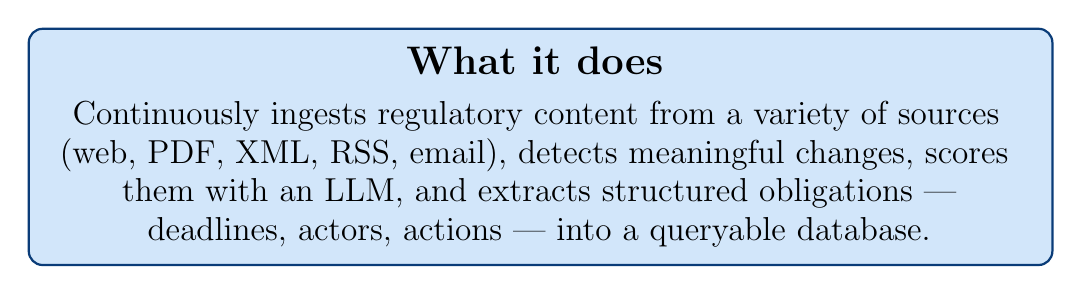
\begin{tikzpicture}
  \node[draw=accent, thick, rounded corners=5pt, fill=accentlight,
        minimum width=13cm, minimum height=3cm, align=center] (box) {
    \parbox{12cm}{\centering
      \Large\textbf{What it does}\par\vspace{4pt}
      \large
      Continuously ingests regulatory content from a variety of
      sources (web, PDF, XML, RSS, email), detects meaningful changes,
      scores them with an LLM, and extracts structured obligations
      ---{} deadlines, actors, actions ---{} into a queryable database.
    }
  };
\end{tikzpicture}

\vspace{1.2cm}

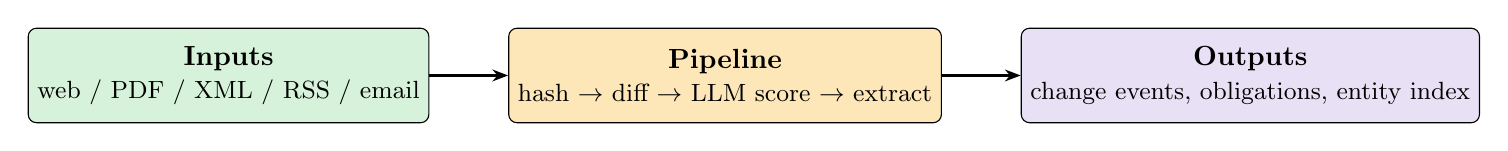
\begin{tikzpicture}
  \node[draw, rounded corners=3pt, fill=L2, minimum width=3.2cm, minimum height=1.2cm, align=center] (in) {\textbf{Inputs}\\{\small web / PDF / XML / RSS / email}};
  \node[right=1.0cm of in, draw, rounded corners=3pt, fill=L3, minimum width=3.2cm, minimum height=1.2cm, align=center] (proc) {\textbf{Pipeline}\\{\small hash $\to$ diff $\to$ LLM score $\to$ extract}};
  \node[right=1.0cm of proc, draw, rounded corners=3pt, fill=L4, minimum width=3.2cm, minimum height=1.2cm, align=center] (out) {\textbf{Outputs}\\{\small change events, obligations, entity index}};
  \draw[-{Stealth[length=2mm]}, thick] (in) -- (proc);
  \draw[-{Stealth[length=2mm]}, thick] (proc) -- (out);
\end{tikzpicture}

\vfill
{\small
Project: \texttt{regulation-prj-v1} \quad $\cdot$ \quad
Stack: Python 3.11, FastAPI, Celery, PostgreSQL 16, Redis 7 \\
LLM: OpenAI \texttt{gpt-4o-mini} (JSON mode, temperature 0) \\
Date: \today
}
\end{titlepage}

% ── TOC ──
\tableofcontents
\newpage

% =========================================================================
\section{The problem}

Regulated businesses (banks, importers, pharma, data-processors) have
to continuously track rule changes across dozens of authorities, each
publishing through different channels (websites, PDFs, RSS feeds, XML
bulk dumps, email bulletins). Today this work is done either by
armies of analysts reading PDFs, or by brittle scripts that break the
moment a web page is rebranded.

Regulatory Watch replaces that with an always-on pipeline that
answers three questions for every piece of regulatory content:

\begin{enumerate}[leftmargin=1.4em,itemsep=2pt]
  \item \textbf{Has anything changed since the last check?} ---{}
        deterministic, content-hash based.
  \item \textbf{Does the change actually matter?} ---{}
        LLM-scored on a 0--1 significance scale with a change-type
        taxonomy (\emph{typo / minor wording / clarification /
        substantive / critical}).
  \item \textbf{What concrete obligations does it impose?} ---{}
        structured rows of \emph{(actor, action, condition, deadline,
        penalty)} extracted from the text and persisted to the DB.
\end{enumerate}

Downstream applications (alerts, dashboards, personalised digests,
integrations with risk-management systems) read from those same
structured tables ---{} they never have to parse HTML themselves.

% =========================================================================
\section{High-level architecture}

\subsection{Component map}

\begin{center}
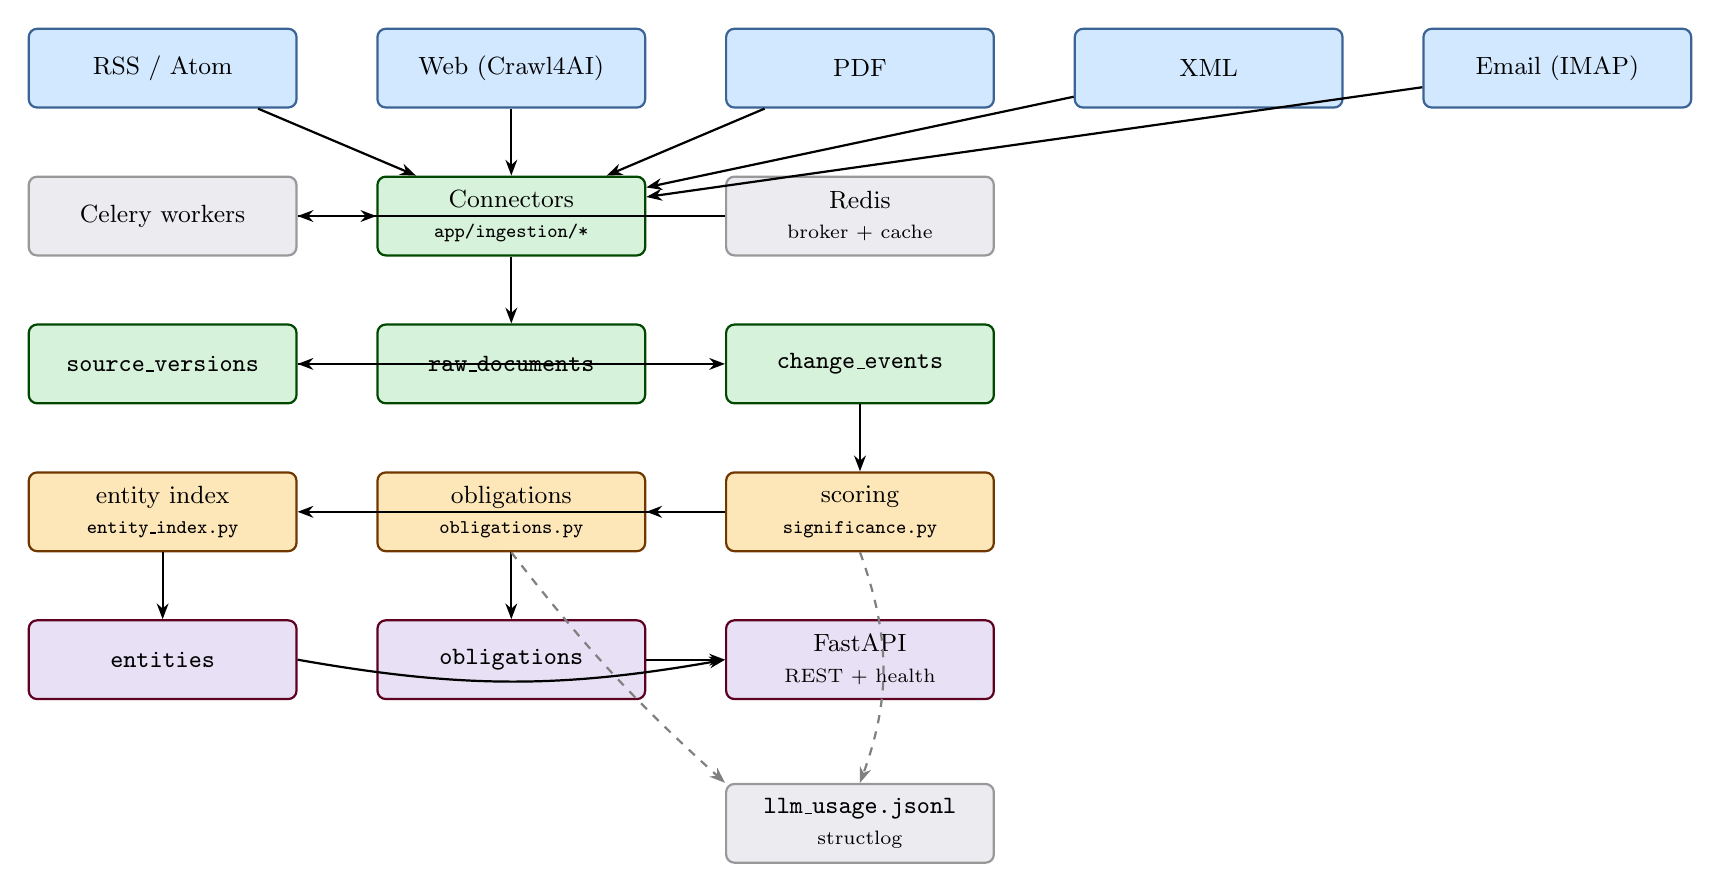
\begin{tikzpicture}[
  node distance=0.85cm and 1.0cm,
  stage/.style={draw, thick, rounded corners=3pt, minimum width=3.4cm,
                minimum height=1.0cm, align=center, font=\small},
  src/.style={stage, fill=L1, draw=accent!80},
  store/.style={stage, fill=L2, draw=ok!60!black},
  llm/.style={stage, fill=L3, draw=warn!70!black},
  ops/.style={stage, fill=L5, draw=black!40},
  down/.style={stage, fill=L4, draw=purple!50!black},
  arr/.style={-{Stealth[length=2mm]}, thick},
  dasharr/.style={arr, dashed, gray},
]

% Row 1 — sources
\node[src] (rss)   {RSS / Atom};
\node[src, right=of rss] (web) {Web (Crawl4AI)};
\node[src, right=of web] (pdf) {PDF};
\node[src, right=of pdf] (xml) {XML};
\node[src, right=of xml] (email){Email (IMAP)};

% Row 2 — connectors
\node[store, below=of web] (connectors) {Connectors \\ {\scriptsize \texttt{app/ingestion/*}}};
\node[ops, left=of connectors] (celery) {Celery workers};
\node[ops, right=of connectors] (redis) {Redis \\ {\scriptsize broker + cache}};

% Row 3 — pipeline stores
\node[store, below=of connectors] (rawdoc) {\texttt{raw\_documents}};
\node[store, left=of rawdoc] (srcver) {\texttt{source\_versions}};
\node[store, right=of rawdoc] (cevent) {\texttt{change\_events}};

% Row 4 — LLM services
\node[llm, below=of cevent] (score) {scoring \\ {\scriptsize \texttt{significance.py}}};
\node[llm, left=of score] (obl) {obligations \\ {\scriptsize \texttt{obligations.py}}};
\node[llm, left=of obl] (ent) {entity index \\ {\scriptsize \texttt{entity\_index.py}}};

% Row 5 — downstream
\node[down, below=of obl] (obls) {\texttt{obligations}};
\node[down, left=of obls] (entities) {\texttt{entities}};
\node[down, right=of obls] (api) {FastAPI \\ {\scriptsize REST + health}};

% Observability
\node[ops, below=of api, yshift=-0.2cm] (ledger) {\texttt{llm\_usage.jsonl} \\ \scriptsize structlog};

% Connections
\foreach \s in {rss,web,pdf,xml,email} { \draw[arr] (\s) -- (connectors); }
\draw[arr] (celery) -- (connectors);
\draw[arr] (redis) -- (celery);
\draw[arr] (connectors) -- (rawdoc);
\draw[arr] (rawdoc) -- (srcver);
\draw[arr] (srcver) -- (cevent);
\draw[arr] (cevent) -- (score);
\draw[arr] (score) -- (obl);
\draw[arr] (score) -- (ent);
\draw[arr] (obl) -- (obls);
\draw[arr] (ent) -- (entities);
\draw[arr] (obls) -- (api);
\draw[arr] (entities.east) to[bend right=10] (api.west);

\draw[dasharr] (score.south) to[bend left=20] (ledger.north);
\draw[dasharr] (obl.south) to[bend right=5] (ledger.north west);
\end{tikzpicture}
\end{center}

\subsection{Three layers, one pipeline}

\begin{center}
\small
\begin{tabularx}{\linewidth}{@{}lX@{}}
\toprule
\textbf{Layer} & \textbf{Responsibility} \\
\midrule
\textbf{L1 Ingestion} &
Poll / crawl each source on a schedule. Normalise text,
de-duplicate, persist \texttt{RawDocument}. One connector per
channel. Deterministic, no LLM. \\
\textbf{L2 Versioning \&} &
For every unchanged-URL re-fetch, compute SHA-256 on the
normalised text. If it differs from the previous
\texttt{SourceVersion}, persist the new version and emit a
\texttt{ChangeEvent}. Still deterministic, no LLM. \\
\textbf{change detection} & \\
\textbf{L3 Significance \&} &
Ask an LLM the compliance-officer question: \textit{does this
matter?} Record score (0--1), change-type, topic,
affected entities, short summary. \\
\textbf{enrichment} & \\
\textbf{L4 Obligations \&} &
For high-significance events ($score \geq 0.6$), extract
structured obligations (actor, action, deadline, penalty,
type). Sync entity index across events. \\
\textbf{entity index} & \\
\bottomrule
\end{tabularx}
\end{center}

Each layer is designed so the one below it can fail without blocking
the one above: a stale LLM doesn't stop ingestion, a broken
connector doesn't stop scoring for other sources.

% =========================================================================
\section{Data model}

\begin{center}
\small
\begin{tabularx}{\linewidth}{@{}lX@{}}
\toprule
\textbf{Table} & \textbf{Purpose} \\
\midrule
\texttt{domains}             & Seed registry: one row per regulator, holds rate-limit \& schedule policy. \\
\texttt{urls}                & Discovered URLs under a domain with priority, relevance and back-off state. \\
\texttt{fetch\_runs}          & One row per scheduled crawl (success / fail / counts). \\
\texttt{fetch\_attempts}      & One row per URL within a run (HTTP status, content hash, timings). \\
\midrule
\texttt{raw\_documents}       & Latest content per source URL (web / pdf / rss / xml / email). \\
\texttt{source\_versions}     & Append-only version log keyed by \texttt{(source\_url, content\_hash)}. \\
\texttt{change\_events}       & One row per detected change; carries LLM score, topic, summary. \\
\midrule
\texttt{entities}            & Canonical entity registry (agencies, regulations, codes...). \\
\texttt{change\_event\_entities}& Many-to-many join of events $\leftrightarrow$ entities. \\
\texttt{obligations}         & Structured \emph{(actor, action, deadline, penalty, type)} rows. \\
\bottomrule
\end{tabularx}
\end{center}

\subsection{Relationships (simplified)}

\begin{center}
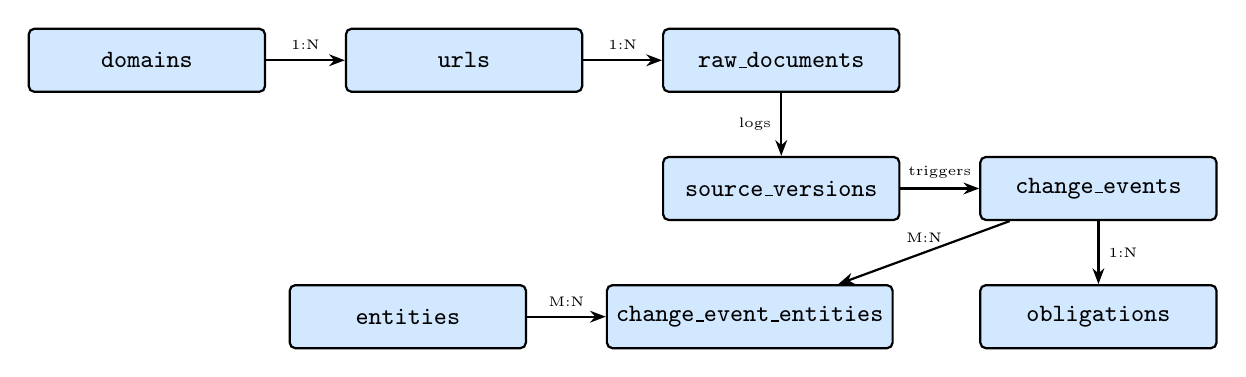
\begin{tikzpicture}[
  entity/.style={draw, thick, rounded corners=2pt, fill=L1, font=\small\ttfamily,
                 minimum width=3.0cm, minimum height=0.8cm, align=center},
  arr/.style={-{Stealth[length=2mm]}, thick},
]
\node[entity] (dom) {domains};
\node[entity, right=1cm of dom] (url) {urls};
\node[entity, right=1cm of url] (raw) {raw\_documents};
\node[entity, below=0.8cm of raw] (ver) {source\_versions};
\node[entity, right=1cm of ver] (evt) {change\_events};
\node[entity, below=0.8cm of evt] (obl) {obligations};
\node[entity, below=0.8cm of ver, xshift=-0.4cm] (x) {change\_event\_entities};
\node[entity, left=1cm of x] (ent) {entities};

\draw[arr] (dom) -- node[above,font=\tiny]{1:N} (url);
\draw[arr] (url) -- node[above,font=\tiny]{1:N} (raw);
\draw[arr] (raw) -- node[left,font=\tiny]{logs} (ver);
\draw[arr] (ver) -- node[above,font=\tiny]{triggers} (evt);
\draw[arr] (evt) -- node[right,font=\tiny]{1:N} (obl);
\draw[arr] (evt) -- node[above,font=\tiny]{M:N} (x);
\draw[arr] (ent) -- node[above,font=\tiny]{M:N} (x);
\end{tikzpicture}
\end{center}

% =========================================================================
\section{The pipeline in detail}

\subsection{Stage 1 --- Ingestion (L1)}

Five connectors, one per channel, all under \texttt{app/ingestion/}:

\begin{center}
\small
\begin{tabularx}{\linewidth}{@{}lX@{}}
\toprule
\textbf{Connector} & \textbf{How it works} \\
\midrule
\texttt{WebConnector}   & Crawl4AI (headless browser w/ JS) + BFS; fallback to httpx + BeautifulSoup. Anti-bot / blocker detection in 5 languages. \\
\texttt{PDFConnector}   & \texttt{pdfplumber}; captures per-page offsets for citation. \\
\texttt{XMLConnector}   & \texttt{lxml}; streaming for USLM/bulkdata-style XML. \\
\texttt{RSSConnector}   & \texttt{feedparser}; one item $\to$ one document. \\
\texttt{EmailConnector} & IMAP; reads regulatory mailing lists (bulletins, press-releases). \\
\bottomrule
\end{tabularx}
\end{center}

Content extraction (\texttt{web\_extractor.py}) strips boilerplate,
navigation, cookie banners, and produces a stable text shape for
downstream hashing.

\subsection{Stage 2 --- Versioning \& change detection (L2)}

Every fetch is normalised then SHA-256 hashed. The loop is:

\begin{enumerate}[leftmargin=1.4em,itemsep=2pt]
  \item Look up the latest \texttt{SourceVersion} for this URL.
  \item If the hash is identical $\Rightarrow$ bump \texttt{last\_seen\_at},
        no event.
  \item If the hash differs $\Rightarrow$ insert new \texttt{SourceVersion},
        emit a \texttt{ChangeEvent} with diff stats (added chars, removed
        chars, diff kind, unified diff preview), enqueue scoring.
\end{enumerate}

All three paths run under a single Postgres transaction per document
so the store is always consistent.

\subsection{Stage 3 --- Significance scoring (L3)}

\texttt{app/services/significance.py} posts the diff + content to
OpenAI in JSON mode and expects back:

\begin{lstlisting}[style=output]
{
  "score": 0.75,
  "change_type": "substantive",
  "topic": "financial_services",
  "affected_entities": ["Financial Conduct Authority", "PSR"],
  "deadline_changes": ["2026-06-30"],
  "summary": "FCA raises minimum capital thresholds..."
}
\end{lstlisting}

\textbf{Change-type taxonomy} (scale banded to the 0--1 score):

\begin{center}
\small
\begin{tabular}{lll}
\toprule
\textbf{Band}       & \textbf{Type}            & \textbf{Meaning} \\
\midrule
0.00--0.19 & \texttt{typo\_or\_cosmetic} & Whitespace, broken links, punctuation \\
0.20--0.39 & \texttt{minor\_wording}     & Rephrasing with no legal effect \\
0.40--0.59 & \texttt{clarification}      & Explains existing rule more clearly \\
0.60--0.79 & \texttt{substantive}        & Rule, threshold or scope altered \\
0.80--1.00 & \texttt{critical}           & New deadline / penalty / obligation \\
\bottomrule
\end{tabular}
\end{center}

\textbf{Topic taxonomy}: \texttt{customs\_trade},
\texttt{financial\_services}, \texttt{data\_privacy},
\texttt{environmental}, \texttt{healthcare\_pharma},
\texttt{sanctions\_export\_control}, \texttt{labor\_employment},
\texttt{tax\_accounting}, \texttt{consumer\_protection},
\texttt{corporate\_governance}, \texttt{other}.

Everything is fail-soft: on LLM error, the event gets
\texttt{llm\_error} set, a char-count heuristic can still drive
alerts, and the circuit breaker (see below) pauses further calls.

\subsection{Stage 4 --- Obligations \& entity index (L4)}

For events with $score \geq 0.6$, \texttt{obligations.py} asks the
LLM to extract atomic compliance facts. Output is validated against a
Pydantic schema and persisted one row per obligation:

\begin{center}
\small
\begin{tabular}{lll}
\toprule
\textbf{Column} & \textbf{Example}                                      & \textbf{Notes} \\
\midrule
\texttt{actor}           & ``firms offering BNPL agreements'' & \\
\texttt{action}          & ``Extend promotional period\ldots'' & \\
\texttt{condition}       & ``if customer affected by Covid-19'' & \\
\texttt{deadline\_text}  & ``by 30 June 2026''                   & free-text from LLM \\
\texttt{deadline\_date}  & \texttt{2026-06-30}                    & parsed by \texttt{\_parse\_deadline} \\
\texttt{penalty}         & ``up to \pounds1m per breach''                & \\
\texttt{obligation\_type}& \texttt{reporting} / \texttt{prohibition} / \texttt{threshold} / \texttt{disclosure} / \texttt{registration} / \texttt{penalty} / \texttt{other} & CHECK-constrained \\
\bottomrule
\end{tabular}
\end{center}

\texttt{entity\_index.py} normalises each entity mentioned by the LLM
into a canonical form (``FCA'' $\equiv$ ``Financial Conduct
Authority'') so cross-event queries (\emph{``show all high-score
changes touching the FCA in the last 30 days''}) are one SQL away.

% =========================================================================
\section{Resilience \& observability}

\begin{center}
\small
\begin{tabularx}{\linewidth}{@{}lX@{}}
\toprule
\textbf{Concern} & \textbf{Mechanism} \\
\midrule
Failing LLM        & Per-task retry budget + Redis-backed circuit breaker (10 errors / 60\,s $\to$ 5-min cooldown). \\
Overloading OpenAI & Celery rate limits: scoring 60/min, obligations 30/min. \\
Prompt regressions & Every call logs \texttt{request\_hash}, \texttt{latency\_ms} and raw-response on parse failure. \\
Cost drift         & \texttt{llm\_usage.jsonl} ledger with per-call USD cost; CLI report (\texttt{scripts/llm\_cost\_report.py}). \\
DB schema drift    & Alembic is the sole schema writer; \texttt{create\_all()} gated behind a dev flag. \\
Connection pool exhaustion & Explicit SQLAlchemy pool sizing; health checks. \\
Production secrets & Env-vars from vault; \texttt{.env} is dev-only (see \texttt{docs/secrets.md}). \\
Log aggregation    & \texttt{structlog} JSON across API, Celery and services ---{} parseable by Loki, Datadog, CloudWatch. \\
Anti-bot pages     & Multilingual detector + Redis per-domain block counters. \\
\bottomrule
\end{tabularx}
\end{center}

% =========================================================================
\section{API \& operational surface}

\subsection{REST API (FastAPI, \texttt{/docs})}

\begin{center}
\small
\begin{tabular}{lll}
\toprule
\textbf{Method} & \textbf{Path}               & \textbf{Purpose} \\
\midrule
GET    & \texttt{/health}           & Liveness probe \\
GET    & \texttt{/health/db}        & DB + Redis health \\
POST   & \texttt{/domains}          & Register a new regulator source \\
GET    & \texttt{/domains}          & List registered domains \\
GET    & \texttt{/domains/\{id\}}   & Get one domain + policy \\
PATCH  & \texttt{/domains/\{id\}}   & Update rate-limit / status \\
DELETE & \texttt{/domains/\{id\}}   & Remove a domain \\
\bottomrule
\end{tabular}
\end{center}

\subsection{Celery tasks (auto-scheduled by Celery-beat)}

\begin{center}
\small
\begin{tabular}{llr}
\toprule
\textbf{Task}                   & \textbf{Trigger}         & \textbf{Period} \\
\midrule
\texttt{heartbeat}              & Every 60\,s          & liveness   \\
\texttt{rss\_ingest\_task}      & Per registered feed  & 30\,min    \\
\texttt{web\_crawl\_task}       & Per registered seed  & 6\,h       \\
\texttt{pdf\_ingest\_task}      & Ad-hoc / discovered  & on demand  \\
\texttt{xml\_ingest\_task}      & Per bulkdata source  & 24\,h      \\
\texttt{email\_ingest\_task}    & IMAP mailbox         & 15\,min    \\
\texttt{score\_change\_event}   & Auto-enqueued on diff& --         \\
\texttt{extract\_obligations\_task} & After scoring ($\geq 0.6$) & -- \\
\bottomrule
\end{tabular}
\end{center}

\subsection{Operator CLIs}

\begin{center}
\small
\begin{tabularx}{\linewidth}{@{}lX@{}}
\toprule
\textbf{Script} & \textbf{Shows} \\
\midrule
\texttt{scripts/show\_changes.py}     & Recent change events with score, type, topic, URL. \\
\texttt{scripts/show\_entities.py}    & Top entities by mention count (filter by type / score / window). \\
\texttt{scripts/show\_obligations.py} & Structured obligations with deadlines \& actors. \\
\texttt{scripts/score\_backlog.py}    & Re-score unscored / errored events (\texttt{--retry-errors}). \\
\texttt{scripts/llm\_cost\_report.py} & Token + USD report from the ledger. \\
\texttt{scripts/domain\_report.sql}   & Per-domain roll-up of fetches, changes, obligations. \\
\bottomrule
\end{tabularx}
\end{center}

% =========================================================================
\section{Tech stack}

\begin{center}
\small
\begin{tabularx}{\linewidth}{@{}lXl@{}}
\toprule
\textbf{Layer}    & \textbf{Tool}              & \textbf{Why} \\
\midrule
Web API           & FastAPI                    & Pydantic-native, async, OpenAPI out of the box. \\
Async workers     & Celery + Redis             & Battle-tested, per-task rate limits, good ecosystem. \\
Scheduler         & Celery-beat                & Co-located with workers, no extra process. \\
ORM               & SQLModel (SQLAlchemy + Pydantic) & Same model for DB and API. \\
DB                & PostgreSQL 16              & JSONB for entities, CHECK constraints on obligations. \\
Schema migrations & Alembic                    & Sole schema writer (no \texttt{create\_all}). \\
Web crawling      & Crawl4AI (Playwright)      & Renders JS, markdown output. \\
HTML fallback     & httpx + BeautifulSoup      & Lightweight, JS-free pages. \\
PDF               & pdfplumber                 & Per-page offsets (citations). \\
XML / feeds       & lxml + feedparser          & Stream-friendly. \\
LLM               & OpenAI \texttt{gpt-4o-mini} & JSON mode, cheap, deterministic. \\
Logging           & structlog                  & JSON for aggregators. \\
Tests             & pytest + freezegun + fakeredis & 93 unit tests, $\sim$0.65\,s. \\
Deploy            & Docker Compose             & \texttt{api}, \texttt{worker}, \texttt{flower}, \texttt{db}, \texttt{redis}, \texttt{kafka}, \texttt{zookeeper}. \\
\bottomrule
\end{tabularx}
\end{center}

% =========================================================================
\section{Economics}

\textbf{Marginal cost per event} (measured from a live run):

\begin{center}
\small
\begin{tabular}{lrr}
\toprule
\textbf{Event type}                         & \textbf{Tokens} & \textbf{USD} \\
\midrule
Low-significance (scored, no obligations)   & $\sim$2{,}100   & \$0.000346 \\
High-significance (scored + obligations)    & $\sim$4{,}200   & \$0.000725 \\
\midrule
1{,}000 events / month                       &                 & \$0.72 \\
10{,}000 events / month                      &                 & \$7.25 \\
100{,}000 events / month                     &                 & \$72.50 \\
\bottomrule
\end{tabular}
\end{center}

The LLM is a rounding error compared to crawler and database infra
costs even at moderate scale. The 0.6 score-gate cuts the
obligations spend by $\sim$60\% and hard token caps
(\texttt{LLM\_MAX\_*} in config) prevent a single runaway document
from blowing the budget.

% =========================================================================
\section{Current status}

\begin{itemize}[leftmargin=1.4em,itemsep=2pt]
  \item \textbf{M1 --- single-source ingestion:} complete.
  \item \textbf{M2 --- multi-source ingestion (5 connectors):} complete.
  \item \textbf{M3 --- versioning + change detection + LLM scoring:} complete.
  \item \textbf{M4 --- obligations + entity index (LLM-only):} complete.
  \item \textbf{Professionalism pass:} complete
        (12/12 items, 93 unit tests passing).
  \item \textbf{Token \& cost observability:} complete
        (ledger + CLI report + per-call USD).
\end{itemize}

\noindent\textbf{Polish items queued} (not blocking pilot):
CI (GitHub Actions) running the test suite on every push;
Prometheus metrics + \texttt{/metrics} endpoint;
end-to-end integration test covering crawl $\to$ score $\to$
obligations in one run;
prompt refinement so past-meeting dates aren't misread as compliance
deadlines.

\vspace{0.5cm}
\begin{center}
\small\itshape
Source: \texttt{regulation-prj-v1} --- see
\texttt{docs/product\_overview.tex} to regenerate this document.
\end{center}

\end{document}
